%
% Chapter 5
%

\chapter{Event Reconstruction}
\label{chap:event_reco}

This chapter begins with the description of the particle-flow algorithm followed by the reconstruction of tracks and vertices, electrons, muons, jets, and other physics objects.

\section{Particle flow}
\label{p_flow}
The global event reconstruction (also called particle-flow (PF) event reconstruction ~\cite{Sirunyan:2017ulk}) aims to reconstruct and identify each particle in an event with an optimized combination of information from the various elements of the CMS detector. In this process, the identification of the PF candidate type (photon, electron, muon, charged, and neutral hadrons) plays a vital role in determining particle direction and energy. The PF algorithm links several PF elements that a physics object can give rise to, across different sub-detector layers. The PF elements are tested for their compatibility in the $\eta-\phi$ plane and are combines to form PF blocks. A predefined sequence of reconstruction and identification algorithms are run in each of these PF blocks. This sequence starts with the reconstruction and identification of muon candidates. PF quality criteria are placed for the muon candidate. The PF elements associated with a muon candidate passing these criteria are removed from the block. The next step in the sequence is to reconstruct and identify electron candidates. The electron candidates are defined as PF electrons if the extrapolated tracks from the tracker have a corresponding energy deposit in the ECAL. The sequence now proceeds with identifying photons and hadrons. At this stage in the sequence tracks with momentum uncertainty more than the resolution of the calorimeters are removed to reduce fake track identification. All the remaining tracks are associated with charged hadrons, and all the remaining calorimeter energy deposits are associated with photons (ECAL) and hadrons (HCAL). At the end of this sequence, we are left with a list of all electrons, photons, muons, charged hadrons, and neutral hadrons in the event with optimally determined direction, charge, and energy.

\section{Track and primary vertex reconstruction}
\label{track_recon}

The hits from the pixel and strip detectors in the tracker are used to reconstruct the tracks of charged particles ~\cite{Chatrchyan:2014fea}. Signals above specified thresholds in the pixel and strip channels are clustered to form the hits. The cluster positions and corresponding uncertainties are estimated in a local orthogonal system plane of each sensor. A translation is done between the local coordinate system of these hits to the global coordinate system of the tracks during track reconstruction. Kalman filter ~\cite{Fruhwirth:1987fm} based algorithm is used to reconstruct tracks and is called the Combinatorial Track Finder (CTF). Tracks with high \pt and those that are produced near the interaction region are easiest to find. Track reconstruction uses an iterative procedure with the initial iterations searching for the most accessible tracks. In subsequent iterations, tracks with low \pt and those produced far from the interaction region are searched. Hits unambiguously assigned to the track in the previous iterations are removed. This reduces the combinatorial complexity in the subsequent iterations. In each iteration, there are four sequential steps.

The first step in the sequence is seed generation. The magnetic field causes the charged particles to follow a helical path, thus requiring five parameters to determine the trajectory. These parameters are extracted using two or three hits in the inner region of the tracker. The seeds are constructed in the inner part owing to the high granularity of the pixel detectors. The tracks are then constructed outwards. The motivation to use the inner region for seed construction also rests on the fact that particles like pions and electrons interact inelastically with tracker material as they traverse through the tracker to its outer regions.

Kalman filter-based algorithm is then used for track finding. Track parameters are estimated by using the trajectory seeds generated in the previous step. The seed trajectories are extrapolated along the expected path of a charged particle. The track candidates are built using the location and uncertainty of detected hits, also taking into account effects such as Coulomb scattering at successive detector layers. The parameters are updated at each layer. An analytical extrapolation is done that determines which adjacent layers of the detector the trajectory can intersect. A search is performed for silicon modules in these layers that are compatible with the extrapolated trajectory. Mutually exclusive groups are built from all compatible modules in each layer such that no two modules in each group overlap. One of the compatible hits from a group of hits is added to the original track candidate to form new track candidates. The information from the added hits is combined with the original track candidates' extrapolated trajectory to update the trajectory parameters of the new candidates. Figure ~\ref{fig:trackrecon} illustrates the reconstruction efficiency of tracks in the case of isolated muons.

The collection of hits from the last step are refitted using a Kalman filter in a phase called track fitting. This provides the best possible estimate of parameters for each track trajectory. There can be several fake tracks that are not associated with any charged particle passing through the tracker. Several quality requirements are applied to the set of reconstructed tracks, which substantially reduces the fake contribution. The quality criterion involves the minimum number of layers the track has hits in, how compatible its origin is with a primary vertex, and how good a fit it yields.

\begin{figure*}
  \begin{center}
    \captionsetup{width=0.9\textwidth,justification=centering}
    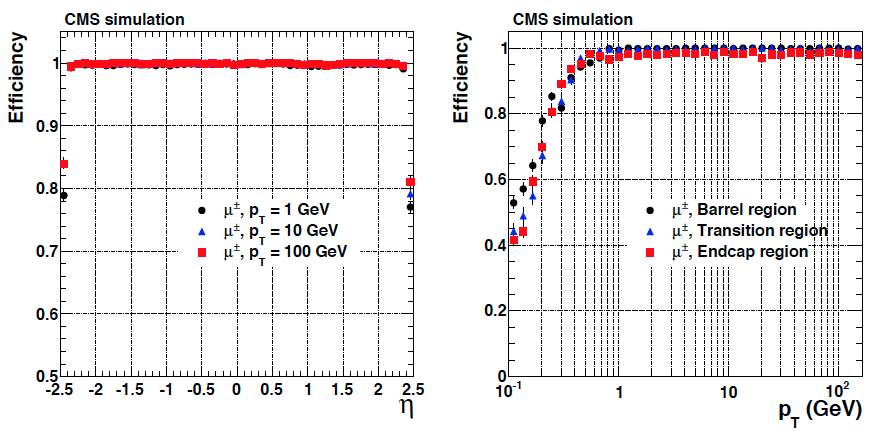
\includegraphics[width=0.9\textwidth,keepaspectratio]{plots/chapter4/trackrecon.png}
    \caption{Track reconstruction efficencies for single isolated muons as a function of $\eta$ and \pt ~\cite{Chatrchyan:2014fea}.}
    \label{fig:trackrecon}
  \end{center}
\end{figure*}

The interaction vertices in the proton-proton collisions are reconstructed by selecting tracks produced promptly in the primary interaction region. The chosen tracks are clustered based on their z-coordinates at their point of closest approach to the center of the beam spot. The beam spot represents a 3-D profile of the region where the proton beams collide inside the CMS detector. The adaptive vertex fitter procedure is used for finding the exact positions of the vertices from these clustered candidates ~\cite{Fruhwirth:2007hz}. The primary interaction vertex has the most significant sum of squared transverse momenta of tracks originating from it.

\subsection{Muon reconstruction}
\label{mu_recon}

Muons are reconstructed using the hits in the muon system and tracks from the tracker ~\cite{Sirunyan:2018fpa}. The gas in the muon chambers is ionized when muons traverse through them. The ionization is read out by electronics systems that associate these ``hits'' with well-defined locations in the detector. The hits in the muon chambers are reconstructed independently of track reconstruction in the tracker. Kalman filter is used for reconstructing the hits from the muon system. These tracks are called \textit{standalone-muon tracks}.
Tracker tracks with transverse momentum above 0.5 GeV are propagated to the muon system. Muon tracks are built from these tracks by matching them to segments of hits in DT or CSC. A matching tracker track is called a \textit{tracker muon track}. Standalone-muon tracks can be matched with tracker tracks and combining information from both using a Kalman filter fit. The muon tacks built in such a manner are called \textit{global muon tracks}. Muons leaving hits in several muon stations have a very efficient global muon reconstruction. Muon candidates with low \pt have an efficient \textit{tracker muon} reconstruction. However, it can cause fake muon tracks due to hadronic particles, which \textit{punch-through} to the innermost muon stations. The \textit{global muon} reconstruction reduces the muon misidentification rate compared to tracker muons. The efficiency for reconstructing a muon is as high as 99\% when \textit{tracker muon tracks} and \textit{global muon tracks} are combined. PF algorithm applies the quality criterion for the reconstructed muon candidates. The PF muon candidates used in the analysis were required to satisfy the following set of criterion to be identified as a muon:

\begin{itemize}
  \item The candidate is reconstructed as a Global Muon along with PF muon identification.
  \item $\chi^{2}$/ndof of the global-muon track fit $<$ 10.
  \item At least one muon-chamber hit included in the global-muon track fit.
  \item Muon segments in at least two muon stations. This implies that the muon is also an arbitrated tracker muon.
  \item Its tracker track has transverse impact parameter $|dxy| < 2$ mm w.r.t. the PV.
  \item The longitudinal distance of the tracker track wrt. the PV is $|dz| < 5$ mm.
  \item Number of pixel hits $>$ 0.
  \item Number of tracker layers with hits $>$ 5.
\end{itemize}

PF muon identification efficiency is illustrated using a plot from a study performed by the CMS Muon Physics Object group in Figure ~\ref{fig:muoneff}. There are differences in the efficiencies in data and MC simulation. They are corrected using a set of scale-factors applied as a function $\eta$ and \pt to adjust the efficiency in simulation to get it to match the efficiency in data.

\begin{figure*}[!htpb]
  \centering
  \captionsetup{width=0.98\textwidth,justification=centering}
  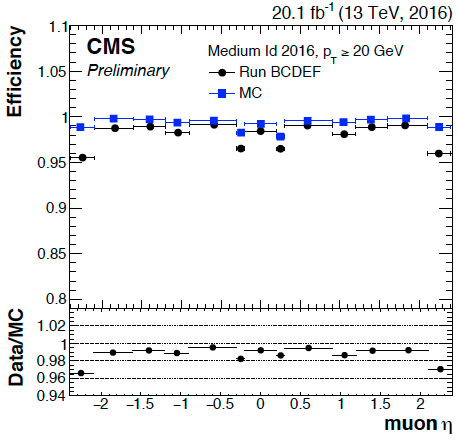
\includegraphics[width=0.47\textwidth]{plots/chapter4/muoneffveta.png}
  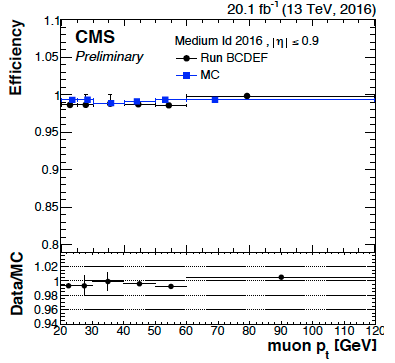
\includegraphics[width=0.49\textwidth]{plots/chapter4/muoneffvpt1.png} \\
  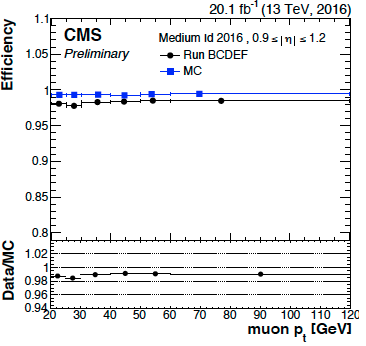
\includegraphics[width=0.49\textwidth]{plots/chapter4/muoneffvpt2.png}
  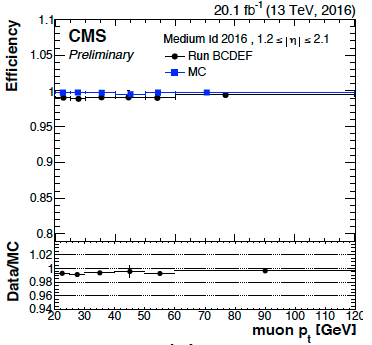
\includegraphics[width=0.49\textwidth]{plots/chapter4/muoneffvpt3.png}
  \caption{Efficiency of muon identification as a function of $\eta$ and \pt, for data (black) and simulation (blue) ~\cite{muon_pog}.}
  \label{fig:muoneff}
\end{figure*}

\subsection{Electron reconstruction}
\label{e_recon}

Clusters of energy formed in the ECAL are associated with tracks from the tracker to reconstruct electrons. Electrons radiate bremsstrahlung photons caused by the interaction of electrons with atoms as they pass through the tracker. The radiation depends on the amount of detector material the electron has to cross. The clustering algorithm needs to account for the energy from these bremsstrahlung photon showers to measure the electron's energy. The energy from the bremsstrahlung photons spreads primarily in the $\phi$ direction, and the spread is $\eta$ direction is relatively small.

The \textit{hybrid} algorithm is used to cluster the electron energy deposit in the ECAL barrel. It uses the geometry of the ECAL to form clusters that are wide in $\phi$ direction but are narrow in $\eta$ direction. A seed crystal contains the most significant amount of energy deposited in the considered region above a 1 GeV threshold. Starting with the seed crystal, 5x1 arrays of crystals are added in $\eta\times\phi$ around the seed crystals in both directions of $\phi$ if the energy contained in the arrays is above 0.1 GeV threshold. Contiguous arrays are merged into clusters. An electron supercluster is formed from all such strip clusters which have at least one seed strip with energy above 0.35 GeV threshold. A different clustering algorithm is used in the ECAL endcap owing to the different geometrical arrangements of the crystals. This algorithm is called the 5x5 algorithm. It starts with a seed crystal satisfying the minimum energy requirement of 0.18 GeV. A supercluster is formed by progressively grouping clusters of 5x5 crystals around the seed crystal. The added clusters need to have energy in excess of 1 GeV and to be within $\pm 0.7$  and $\pm 0.3$ respectively in $\eta$ and $\phi$ around the seed crystal. The energy-weighted mean of the cluster positions is taken as the position of the supercluster. The sum of the energy of all its constituent clusters is its energy. The energy from the preshower is also added to the supercluster. This is implemented by using it's most energetic cluster, and it's maximum distance in $\phi$ to other clusters, and extrapolating it to the preshower plane to define the spread in the preshower.

A dedicated tracking procedure is used for electron candidates that use information not only from the tracker but also from the ECAL. The first step in electron track reconstruction is seeding. The position and energy of the reconstructed superclusters can be used to constrain the trajectory of the electron through the tracker and the assumption that the electrons originated close to the center of the beam spot. The electron seeds are the hits in the first layers of the trackers compatible with these trajectories. In an alternative approach, tracks constructed by the regular tracking algorithm are extrapolated to the ECAL and matched with a supercluster. The seed collections from these two approaches are merged, leading to an increase in the seeding procedure's overall efficiency. Electron track finding and fitting phases use these seeds. Track finding procedure is adjusted to accommodate tracks that deviate from their expected trajectory because of bremsstrahlung. The penalties assigned to track candidates for passing through a tracker layer without being assigned a hit are similarly adjusted. The Gaussian Sum Filter (GSF) is used for the final track fit. This accounts for the fact that the energy loss of an electron traversing the tracker material is non-Gaussian. As the Kalman filter algorithm assumes Gaussian distribution, the GSF technique deals with this by approximating this non-Gaussian energy-loss distribution as the sum of several Gaussian functions and is found to perform much better than the regular fitting procedure.

The electron candidates are constructed by associating the GSF track produced by the above procedure with a supercluster in the ECAL. A geometrical matching in $\eta-\phi$ is used for the association for ECAL-seeded candidates. A multivariate (MVA) technique that combines information from supercluster and GSF track is used for tracker-seeded candidates. The charge of the electron is estimated using the GSF track curvature, ECAL supercluster's relative position in $\phi$ to that of the first hit in the GSF track, and also by using KF tracks that have common hits with the GSF tracks. This combined approach reduces the charge misidentification probability to 1.5\%. A combination of tracker and ECAL measurements is used for estimating the momentum of electrons.

Several quality criteria are placed on the reconstructed electron candidates to identify electrons. This helps in suppressing fake sources such as photon conversions, jets misidentified as electrons, etc. Electrons are required to pass an identification variable based on a Boosted Decision Tree (BDT) discriminator, which uses track quality, shower shapes, and kinematic quantities. The following variables are used as input to the BDT:
\begin{itemize}
  \item Cluster shape variables $\sigma_{i\eta,i\eta}$ and $\sigma_{i\phi,i\phi}$, with i$\eta$ and i$\phi$ the integer label of the $\eta$ and $\phi$ of a calorimeter cell. The circularity = 1 - $\frac{E_{1 \times 5}}{E_{5 \times 5}}$, with $E_{1 \times 5}$ and $E_{5 \times 5}$ the energies in a 1$\times$5 and a 5$\times$5 grid around the super cluster seed, respectively.
  \item Shape variable R9 = $\frac{E_{3 \times 3}}{E_{SC}}$, with $E_{3 \times 3}$ the energy in a 3$\times$3 grid of cells around the super cluster seed and $E_{SC}$ the raw energy of the super cluster.
  \item The number of valid hits in the track fit, the $\chi^{2}$ of the track fit, and the $\chi^{2}$ of the GSF Track fit.
  \item The number of GSF track hits, the number of expected missing inner hits, and the result of the conversion vertex fit.
  \item The distance $\Delta \eta$ and $\Delta \phi$ between the reconstructed supercluster and the associated track at the position of the PV, and the distance in $\eta$ between the supercluster and the track at the calorimeter surface.
  \item H/E, the ratio of the hadronic energy over the electromagnetic energy in the supercluster and E/P, the ratio of the supercluster energy over the momentum of the track associated with the electron.
  \item The ratio of the energy of the electron cluster and the momentum of the associated track, evaluated at the electron cluster, and $1/E_{\Pe} - 1/P_{\Pe}$, with $E_{\Pe}$ the energy of the electron candidate and $P_{\Pe}$ its momentum.
\end{itemize}

Electrons are required to pass an identification variable based on a Boosted Decision Tree (BDT) discriminator, which uses track quality, shower shapes, and kinematic quantities as input. The BDT was trained on a \PZ/\Pgg Monte Carlo sample generated with MadGraph5, in 3 $\eta$ bins for electrons with $\pt > 10$ GeV. Instead of using fixed cuts on the MVA score, the cuts are alternatively varied exponentially with \pt to achieve a more constant efficiency. The tight and loose working points (WPs) are again tuned to give 80\% and 90\% efficiency, respectively.

The EGamma POG provided two versions of the electron ID, one which includes the electron isolation in the training and one which does not include this. This analysis uses the version of the ID without the isolation included in the training. An additional selection of electron isolation is used. This is done so that in the \Hehad channels, the tight-to-loose method for estimating the misidentified lepton background can be implemented, which uses isolation-based sideband regions. The electrons are also subject to the same impact parameter cuts as the muons: the impact parameters between the electron track (best track) and the PV are restricted as $|dxy| < 0.045$ cm and $|dz| < 0.2$ cm to ensure the electron is associated with the PV.

\begin{figure*}[!htpb]
\centering
\captionsetup{width=0.95\textwidth,justification=centering}
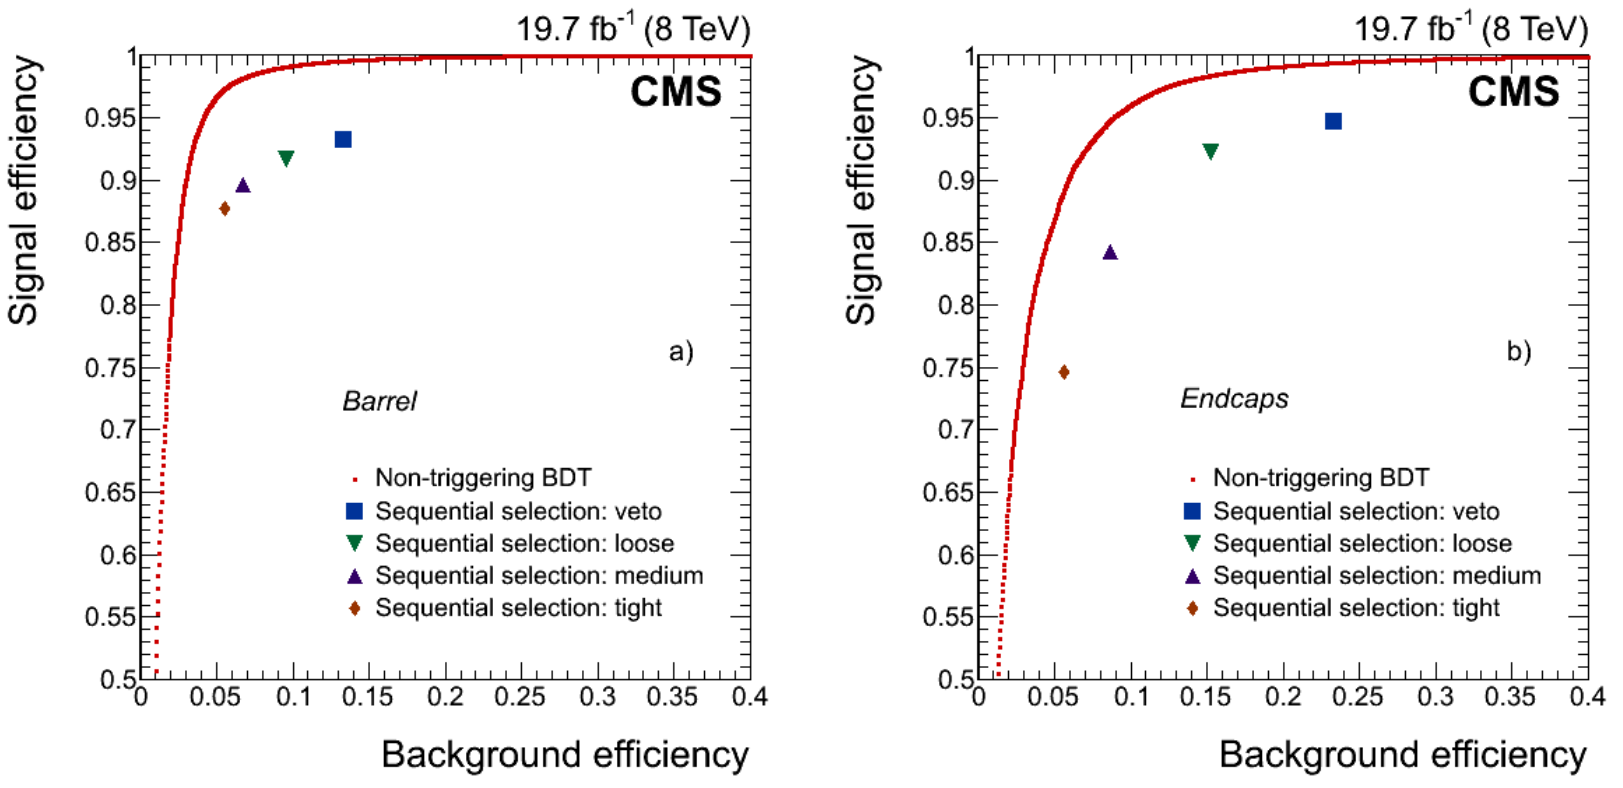
\includegraphics[width=0.95\textwidth]{plots/chapter4/elec_eff.png}
\caption{Performance of the BDT-based electron identification algorithm (red dots) compared with results from several working points of cut-based selection for electron candidates in the ECAL barrel (left), and endcaps (right)~\cite{Khachatryan:2015hwa}.}
 \label{fig:elec_eff}
\end{figure*}

\section{Hadronic tau leptons}
\label{tau_recon}
Hadrons plus strips (HPS) algorithm is used for reconstructing the hadronic decays of tau \cite{Sirunyan:2018pgf}. The Tau POG recommends the use of DeepTau based identification for discrimination against jets, electrons, and muons. A detailed description of the HPS algorithm, followed by the DeepTau Identification algorithm, is given in the following subsections.

\subsection{Hadrons Plus Strips}
\label{sec:tauid_hps}
Taus in the hadrons plus strips algorithm is seeded by jets clustered with the anti-$k_{T}$ algorithm with a distance parameter $\Delta R = 0.4$. To reconstruct the energy deposits \Pgpz candidates leave in the ECAL, photon and electron constituents of the jet that seeds the \tauh reconstruction are clustered into strips. The \Pe or \Pgg (not yet included in a strip) with the highest \pt is used to build a new strip. The $\eta$ and $\phi$ of this candidate determine the initial position of the strip. The next highest \pt \Pe or \Pgg within an $\eta - \phi$ window centered on the strip location is added to the strip. The position is recomputed as the energy-weighted average of the electron/photon constituents in the strip. This procedure is repeated until there are no more electrons or photons with $\pt > 0.5$ GeV within the strip window. The $\Delta \eta $ and $\Delta \phi $ of the strip vary based on the \pt or \ET to be added to the strip. It also depends on the energy, the strip already has, as
\begin{linenomath*}
  \begin{equation*}
    \begin{aligned}
      \Delta \eta = f(\pt^{e/\Pgg}) + f(\pt^{strip}) \\
      \Delta \phi = g(\pt^{e/\Pgg}) + g(\pt^{strip})
    \end{aligned}
  \end{equation*}
\end{linenomath*}
where \pt$^{e/\gamma}$ is the transverse momentum of the candidate to be added to the strip and \pt$^{strip}$ is the transverse momentum of the strip before merging a new candidate in. In addition, the strip size is bounded as 0.05 $< \Delta\eta <$ 0.15, 0.05 $< \Delta\phi <$ 0.3. The functions f(\pt) and g(\pt) are defined as
\begin{linenomath*}
  \begin{equation*}
    \begin{aligned}
      f(\pt) = 0.2 \cdot \pt^{-0.66} \\
      g(\pt) = 0.35 \cdot \pt^{-0.71}
    \end{aligned}
  \end{equation*}
\end{linenomath*}

If the $\pt^{strip}$ is at least 2.5 GeV, it is considered as a \Pgpz candidate. Hadronic taus are reconstructed by combining charged particles and strips into different signatures, which are said to be compatible with a specific DM if the set of cuts listed below is satisfied. If a candidate satisfies more than one of the hypotheses, the one that maximizes the \pt is retained.

The decay modes (DMs) considered for reconstructing taus are:
\begin{itemize}
\item[{\bf One prong, 0 \Pgpz:}] One charged particle, no strips.
\item[{\bf One prong, 1 \Pgpz:}] One charged particle + one strip with mass $0.3 < \mt < 1.3 \cdot \sqrt{\pt/100}$ GeV. The mass window upper limit is constrained to lie between 1.3 and 4.2 GeV.
\item[{\bf Three prong, 0 \Pgpz:}] Three charged particles with mass $0.8 < \mt < 1.5$ GeV. The tracks are required to originate within $|dz| < 0.4$ cm of the same vertex.
\item[{\bf Three prong, 1 \Pgpz:}] Three charged particles and one strip with a total mass $0.8 < \mt < 1.5$ GeV.
\end{itemize}

The reconstructed hadronic tau candidates are subject to the impact parameter cuts: the impact parameter between the reconstructed hadronic tau and the PV is restricted as $|dz| < 0.2$ cm to ensure the hadronic tau is associated with the PV.

\subsection{DeepTau}
\label{sec:tauid_dt}
The application of Machine Learning techniques has been proven to provide superior results for multi-dimensional problems. DeepTau is a new multiclass tau identification algorithm based on a convolutional deep neural network (DNN). DeepTau combines information from the high-level variables attributed to the reconstructed \tauh candidates with low-level information from the inner tracker, calorimeters and muon sub-detectors using PF candidates reconstructed within the \tauh signal and isolation cones. DeepTau also takes advantage of using the updated DM definitions.

A balanced mix of \taue, \taum, \tauh, and \tauj candidates coming from \ttbar, \wjets, and \zjets Monte Carlo (MC) simulation is used to perform the training. The \tauh has a loose preselection: \pt $\in$ [20, 1000] GeV, $|\eta| < 2.3$, and $|dz| < 0.2$, which makes it suitable for the current analysis. The inputs are separated into sets of high-level and low-level features. As high-level inputs, the algorithm takes variables used during tau reconstruction, and one global event variable is the average energy deposition density ($\rho$). For each candidate reconstructed within the tau signal or isolation cones, information of 4-momentum, track quality, relation with the PV, calorimeter clusters, and muon stations are used.

The tau signal and isolation cones define two regions of interest in the vicinity of the tau candidate. Based on the angular distance between the reconstructed tau 4-momentum, all available candidates are split into two $\eta \times \phi$ grids of 11 $\times$ 11 (21 $\times$ 21) cells with a cell size of 0.02 $\times$ 0.02 (0.05 $\times$ 0.05) for the signal (isolation) cone. In cases where there is more than one object of the given type that belong to the same cell, only the object with the highest \pt is considered as input. Within each cell, the input variables are split into three blocks: e-gamma, muon, hadrons.

The organization of the low-level inputs into two 2D grids allows first processing the local patterns originating from the tau or jet structure. The information obtained is then iteratively combined, covering bigger $\eta \times \phi$ regions up to the point where the total tau signal or isolation cones are covered. The four outputs of the network represent estimates of the probabilities of the reconstructed tau candidate to be \taue, \taum, \tauj, or a genuine \tauh. The performance of tau discrimination against quark and gluon induced jets (left), electrons(middle), and muons(right) for DeepTau and the previously available discriminators can be seen in Figure ~\ref{fig:deeptau}.

\begin{figure}[hbtp]
  \centering
  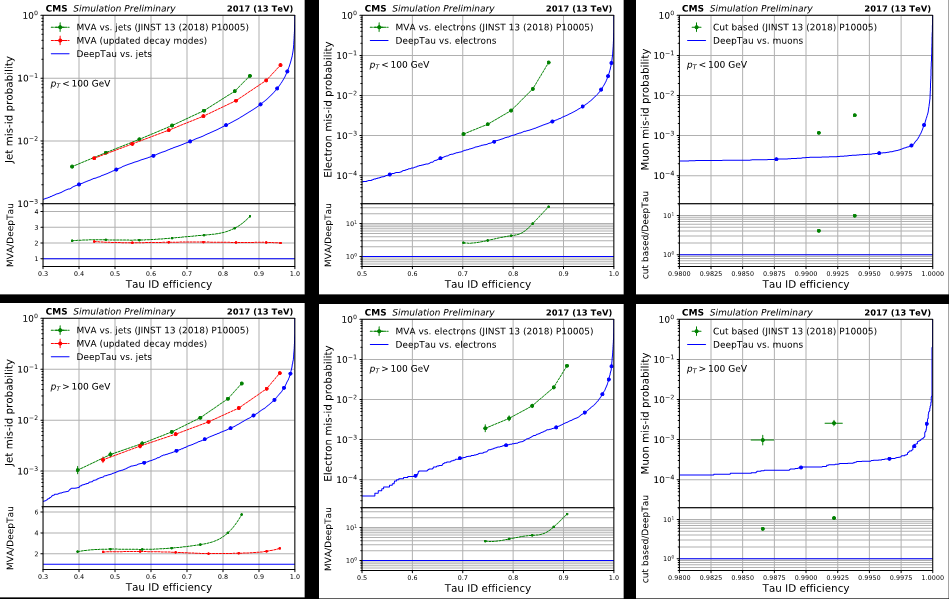
\includegraphics[width=0.9\textwidth]{plots/chapter5/deeptau.png}
  \caption{Performance of tau discrimination against quark and gluon induced jets (left), electrons(middle), and muons(right) for DeepTau and the previously available discriminators}
  \label{fig:deeptau}
\end{figure}

Seven WPs ranging from Very Very Loose to Very Very Tight, are provided. The Tight \tauh WP of the DeepTau discrimination against jets is used to provide good tau efficiency and jet rejection. To reduce the $\Pe\to\tauh$ and $\Pgm\to\tauh$ misidentification, anti-electron, and anti-muon discriminators are used. They are retrieved from the same neural network that is used for the discrimination against jets. The chosen WPs depends on the channel and are specified in the event selection section ~\ref{sec:event_selection}. Eight WPs are provided for the anti-electron discriminator, ranging from Very Very Very Loose to Very Very Tight. Four WPs are provided for the anti-muon discriminator. The choices are made such that efficiency and fake rejection are better than for the WPs chosen in previous analyses for the former discriminators. For anti-muon discriminator, the efficiency hardly changes, so a higher fake rejection is preferred.

\section{Jet reconstruction}
\label{jet_recon}

Quarks and gluons hadronize due to color confinement producing a fine spray of particles called jets ~\cite{Cacciari:2008gp}. Jets are reconstructed using the anti-$k_{T}$ clustering algorithm. This is a sequential clustering algorithm based on the quantities $d_{ij}$, which represents the distance between two entities, and $d_{iB}$, which represents the distance of the i-th object from the beam axis.

These distances are defined as:
\begin{equation}
  d_{ij}=min(k_{ti}^{2p},k_{tj}^{2p})\frac{\Delta_{ij}^{2}}{R^2}
\end{equation}
\begin{equation}
  d_{iB}=k_{ti}^{2p}
\end{equation}
where $\Delta_{ij}^{2}=(\eta_i-\eta_j)^2+(\phi_i-\phi_j)^2$, $k_{ti}$ is the transverse momentum of the i-th entity and R is the radius parameter which is set as 0.4.

In the anti-$k_{T}$ clustering algorithm, $p=-1$, where the parameter p governs the relative power of energy versus geometrical scales. $d_{ij}$ represents the distance between all entity pairs present. If the minimum of those distances is smaller than the minimum distance $d_{iB}$ of any entity from the beam axis, those entities i and j are combined into a single entity. Otherwise, the object closest to the beam axis is considered a jet. It is then removed from the list of entities to be further clustered. The high \pt particles dominate in the anti-$k_{T}$ and are clustered first. Softer constituents are subsequently clustered. Before the soft particles cluster among themselves, they cluster with hard particles. As a result of this, a hard particle with no hard neighbors within a distance 2R accumulates all the soft particles within a circle of radius R. Anti-$k_{T}$ tries to produce jets with somewhat conical shapes are centered around the hardest particles of the event. The boundaries are resilient to the effect of infrared and collinear radiation.

The reconstructed jets' energy differs from their true values as they are complex objects suffering from several effects. Correction factors are applied to calibrate their \pt and to ensure a uniform response in $\eta$ ~\cite{Chatrchyan:2011ds, Khachatryan:2016kdb}. The energy coming from the pileup that has been clustered into the jet needs to be corrected. This is corrected using the \textit{hybrid jet area} method. This method is a combination of the average offset method and the jet area method. The average amount of energy added to the event due to pileup is measured using the zero bias events in the average offset method. This relies on the assumption that averaging over zero bias events makes this measurement insensitive to high \pt objects. The average offset is measured in bins of $\eta$, and the number of pileup vertices ($N_{PV}$) averaged over $\phi$. The correction is then given by $1-\frac{<Offset(N_{PV},\eta)>}{p_{T}^{RAW}}$, where $p_{T}^{RAW}$ is the uncorrected jet \pt. The other assumption is that every jet contains the same amount of pileup contribution, which is a drawback for this method.

The jet area method calculates corrections on a jet-by-jet basis. The energy density per event is calculated by clustering jets using the $k_{T}$ algorithm. The $k_{T}$ algorithm favors clustering soft jets as opposed to hard ones. The \pt is then divided by jet area, which is defined as the region in $\eta-\phi$ occupied by soft particles clustered in the jet. The median of this distribution ($\rho$) for an event is expected to be insensitive to hard particles. This $\rho A_{j}$ is a good approximation of pileup contribution to the i-th jet. However, this approach has a drawback because it doesn't take into account the fact that the detector response is $\eta$ dependent. Thus, the \textit{hybrid jet area} method combines these two methods to calculate a jet-by-jet correction depending on $\eta$ and $N_{PV}$.

The energy of reconstructed jets is corrected with an MC calibration factor to match the generated MC particle jet energy on average. The energy response of reconstructed jets is calibrated to be uniform with respect to $\eta$ and \pt. A QCD dijet sample is used to correct the dependence on $\eta$. Using jets that are approximately back-to-back in the azimuthal direction but at different $\eta$ regions of the detector, the difference in response between these two $\eta$ regions can be ascertained and corrected. Using the same method of measuring residual response in the transverse direction in $\gamma + jets$ or $Z +jets$ events, the absolute jet energy scale as a function of \pt can be made uniform.

\section{Missing transverse energy: \ptvecmiss}
\label{mt_met_recon}
Neutrinos and other hypothetical particles that are weakly interacting cannot be detected in the CMS detector. The momentum imbalance in the transverse plane can be used to infer their presence. The missing transverse momentum vector \ptvecmiss is computed as the negative vector sum of the transverse momenta of all the PF candidates in an event, and its magnitude is denoted as \ptmiss ~\cite{Sirunyan:2019kia}. The \ptvecmiss is modified to account for corrections to the reconstructed jets' energy scale in the event. Anomalous high-\ptmiss events can be due to a variety of reconstruction failures, detector malfunctions, or non-collision backgrounds. Such events are rejected by dedicated filters that are designed to reject more than 85--90\% of the spurious high-\ptmiss events with a signal efficiency of more than 99.9\% ~\cite{Sirunyan:2019kia}. In addition to the event filtering algorithms, the jet identification selection that is imposed requires the neutral hadron energy fraction of a jet to be less than 0.9 rejects more than 99\% of the noise jets, independent of jet \pt, with a negligible mistag rate. Corrections to the \ptvecmiss are applied to reduce the mismodeling of the simulated \zjets, \wjets, and Higgs boson samples. The corrections are applied to the simulated events on the basis of the vectorial difference of the measured missing transverse momentum and total transverse momentum of neutrinos originating from the decay of the \PZ, \PW, or Higgs boson. Their average effect is the reduction of the \ptmiss obtained from the simulation by a few \GeV.

\begin{equation}
  \ptvecmiss=-\Sigma\ptvec
\end{equation}

The \ptvecmiss plays a vital role in this analysis as it helps gauge the momentum of the neutrinos from the decaying tau lepton. The \ptvecmiss reconstruction is directly dependent on the reconstruction of all the other objects in the event, from jets to muons to electrons. Consequently, it is sensitive to all the effects that influence the precise reconstruction and calibration of these objects.

\section{Relative isolation}
\label{isolation}
The muon (electron) isolation is measured relative to its $\pt^\ell (\ell=\Pe,\Pgm)$, by summing over the \pt of PF particles in a cone with $\Delta R=0.4(0.3)$ around the lepton:
\begin{linenomath*}
  \begin{equation*}
    I^\ell_{\text{rel}} = \left( \sum \pt^{\text{PV\;charged}} + \text{max}\left[0, \sum \pt^{\text{neutral}} + \sum \pt^\Pgg - \pt^{\text{PU}}(\ell)\right]\right) \biggm/ \pt^\ell,
  \end{equation*}
\end{linenomath*}
where $\pt^\text{charged}$, $\pt^\text{neutral}$, and $\pt^{\Pgg}$ indicate the \pt of a charged particle, a neutral particle, and a photon within the cone, respectively. The neutral contribution to isolation from pileup, $\pt^\text{PU}(\ell)$, is estimated from the area of the jet and the median energy density of the event ~\cite{Cacciari:2008gn, Cacciari:2007fd} for the electron or from the sum of transverse momenta of charged hadrons not originating from the primary vertex scaled by a factor of 0.5 for the muons. The charged contribution to isolation from the pileup is rejected by requiring the tracks to originate from the PV.

%
% % % uncomment the following lines,
% % if using chapter-wise bibliography
% %
% % \bibliographystyle{ndnatbib}
% % \bibliography{example}
%
% % % uncomment the following lines,
% % if using chapter-wise bibliography
% %
% % \bibliographystyle{ndnatbib}
% % \bibliography{example}
